\chapter{Введение}
\section*{Цель}
Целью данной работы является оптимизация процесса сборки документов системой nutch.
\section*{Nutch}
Nutch - свободное программное обеспечение для интернет поиска.
Nutch основан на поисковом движке Lucene\cite{lucene}, с набором средств для работы с web, таких как поисковый робот, база ссылок, парсеры для html и других форматов и.т.п.
Nutch работает поверх фреймворка hadoop.
\section*{Hadoop}
\label{sec:hadoop}
Hadoop является свободным Java фреймворком, поддерживающим выполнение распределённых приложений, работающих на больших кластерах, построенных на обычном оборудовании. Hadoop прозрачно предоставляет приложениям надёжность и быстродействие операций с данными. В Hadoop реализована вычислительная парадигма, известная как MapReduce.
\section*{MapReduce}
\label{sec:mapred}
Общая идея MapReduce состоит в том, чтобы представить алгоритм в виде набора последовательных этапов, из которых каждый состоит из двух шагов - map и reduce (возможны дополнительные шаги - combine и partition). Система разбивает входные данные на пары $\langle key, value\rangle$, над каждой парой выполняется функция map на выходе которой, должен получится набор пар $\langle key, value\rangle$. 
Сгенерированные данные система реорганизует и для каждого из них выбирает узел на котором исполнится процедура reduce. Данные для одного reduce узла группируются по одинаковым ключам и ключи сортируются. После чего данные, в виде $\langle key, value*\rangle$ опять передаются пользователю, который производит над ними операцию reduce (свёртка) на каждом узле. Получившиеся на выходе пары $\langle key, value\rangle$ передаются в выходной поток (Рис.~\ref{ris:mapreduce}).
  \begin{figure}[h]
    \center{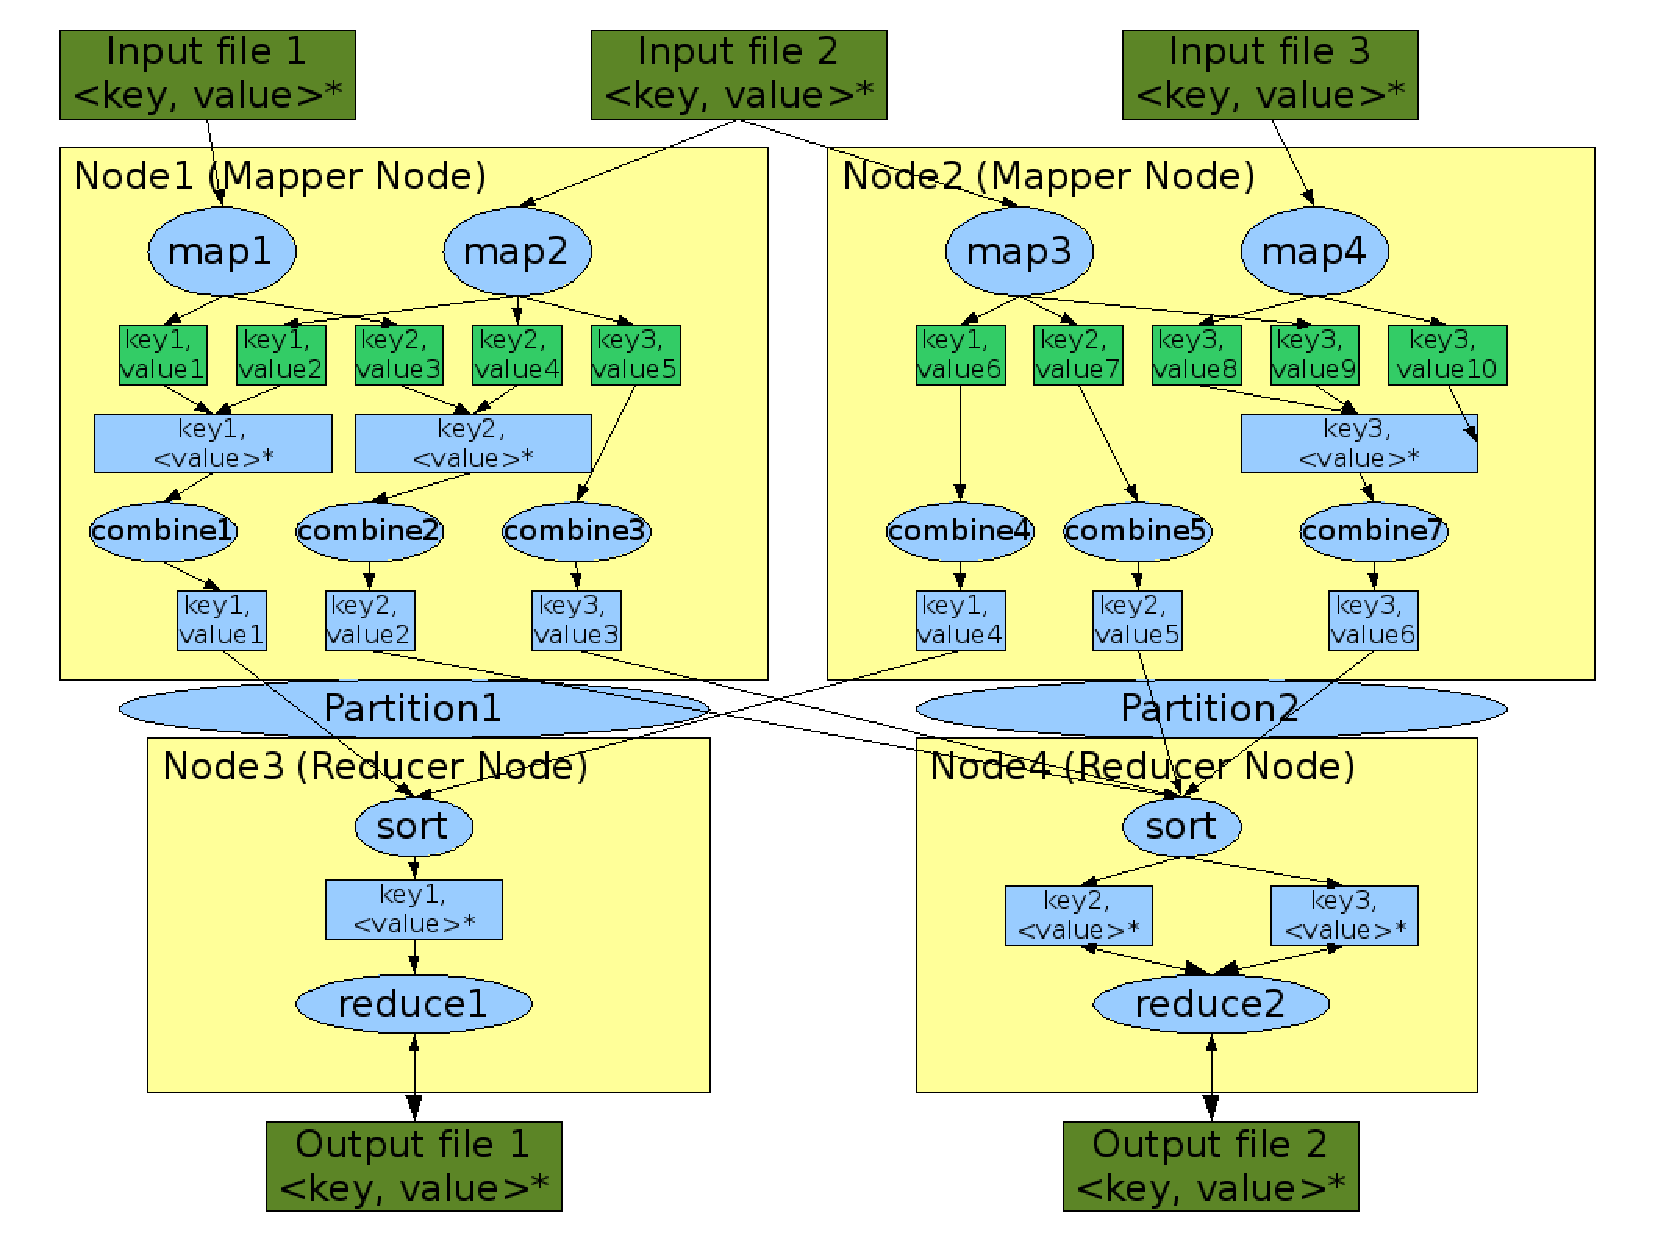
\includegraphics[width=1\linewidth]{img/mapreduce}}
    \caption{Схема MapReduce\cite{pimenov} }
    \label{ris:mapreduce}
  \end{figure}

Преимущество MapReduce заключается в том, что он позволяет распределенно производить операции предварительной обработки и свертки. Операции предварительной обработки работают независимо друг от друга и могут производиться параллельно. Аналогично, множество рабочих узлов могут осуществлять свертку — для этого необходимо только чтобы все результаты предварительной обработки с одним конкретным значением ключа обрабатывались одним рабочим узлом в один момент времени. Таким образом MapReduce может быть применен к большим объемам данных, которые могут обрабатываться большим количеством серверов.\cite{hadoop}
\section*{Работа nutch с точки зрения MapReduce}
Сборка осуществляется итеративно - на каждой итерации осуществляется выбор url для загрузки, загрузка, индексация полученных данных, обновление базы ссылок и обновление базы обратных ссылок. 
  \begin{figure}[h]
    \center{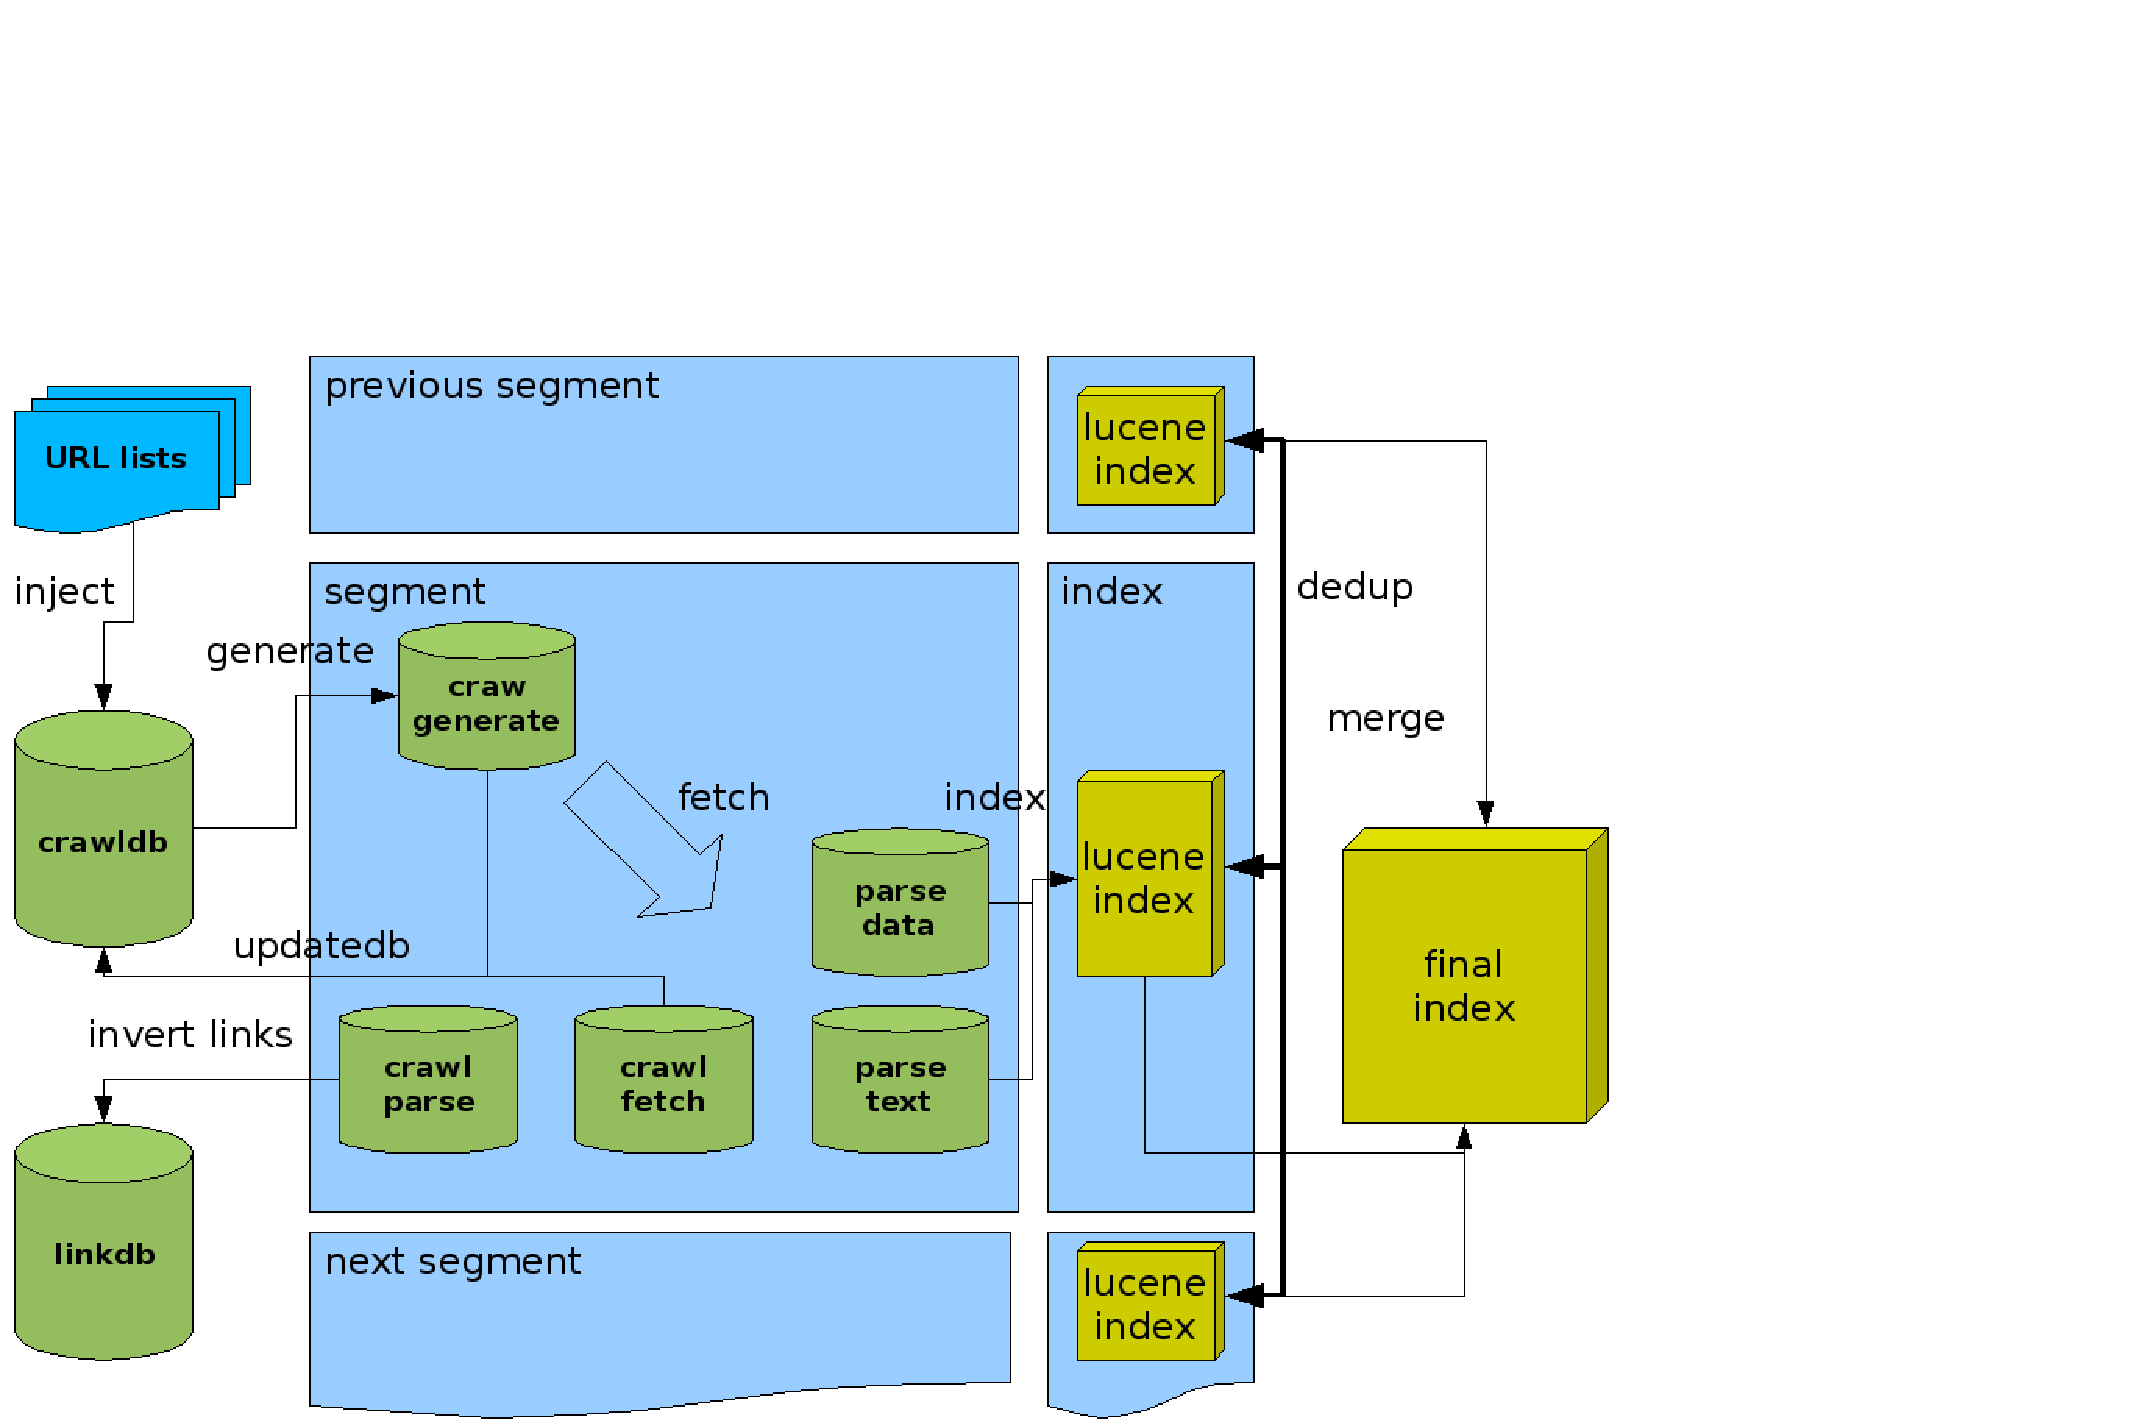
\includegraphics[width=1\linewidth]{img/nutch}}
    \caption{Работа Nutch\cite{pimenov}}
    \label{ris:nutch}
  \end{figure}

На рис. ~\ref{ris:nutch} представлена схема работы nutch, при этом приняты следующие обозначения: 
\begin{itemize}
 \item \texttt{generate} --- выбор url из общей базы (crawldb)
 \item \texttt{fetch} --- загрузка документов по url
 \item \texttt{index} --- создание индекса по скачанным документам
 \item \texttt{merge} --- слияние индекса по сегменту с основным
 \item \texttt{dedup} --- удаление дубликатов из индекса
 \item \texttt{updatedb} --- обновление crawldb
 \item \texttt{invert links} --- создание и обновление базы обратных ссылок (linkdb)

\end{itemize}


\section*{Условия}
Задача web сборки заключается в нахождении нужных url и скачивания документов по ним, большинство url появляется из уже скачанных документов.
Иногда непосредственно по url можно определить что документ является ``полезным''. Например, для того, что бы скачать все новости с ресурса lenta.ru, достаточно скачивать документы по url который можно задать регулярным выражением \ref{eq:lentaregex}

\begin{equation} \label{eq:lentaregex}
http://lenta\textbackslash.ru/news/\textbackslash d\{4\}/\textbackslash d\{2\}/\textbackslash d\{2\}/\textbackslash w+/
\end{equation}
 
\section*{Постановка задачи}
Необходимо изменить nutch для работы с учетом информации о ``полезности'' ссылок.

Основные требования:
\begin{itemize}
 \item минимальные изменения ядра nutch
 \item возможность обновления информации о ссылках без остановки сборки
 \item возможность работы без вмешательства администратора
\end{itemize}
\section*{Актуальность}
Nutch является активно развивающимся проектом, на его основе сейчас создан один из крупнейших поисковиков по исходному коду \href{http://www.krugle.com/}{Krugle}. Одна из основных проблем web-поиска это чрезмерное количество данных. Скачать все даже с одного ресурса крайне ресурсоемкая задача, и даже не всегда выполнимая - т.к. как многие документы создаются динамически, и возможно ``зацикливание''. 

Не смотря на то, что практически каждый ресурс содержит информацию по сборке (robots.txt), не редко огромное количество совершенно бесполезных ссылок и дубликатов не попадает под фильтры, отсюда вытекает необходимость контроля хода сборки в соответствии с дополнительной информацией о url.
